\chapter{Forsøg}
\section{Forsøgsopstillingen}
\begin{figure}[htbp]
    \centering
    \includegraphics[width=0.7\linewidth,origin=c]{figures/Forsøgsopstilling.jpg}
    \caption{Forsøgsopstilling}
    \label{fig:forsøgsopstilling}
\end{figure}
Forsøgsopstillingen består først og fremmest af 1 lod (1), hængt fast til 2 newtonmetrer (5), 
der fungerer som vores fjedrer i systemet. 
De gør det muligt at have en rimelig lineær bevægelse langs overfladen, 
da krogen på newtonmeteret ikke rigtig kan bevæge sig til siden, men kun parallelt med sig selv.
Loddet bevæger sig hen over en overflade (2), der står ovenpå en vægt (3), 
sådan at vi kan måle hvor stor normalkraften mellem loddet og overfladen er.
Vægten står oven på en sakselift, der kan bruges til at øge normalkraften, ved at hæve eller sænke overfladen op i loddet, 
der på grund af newtonmetrerne er nogenlunde stationært i den opadgående retning.
Newtonmetrerne er hængt op på 2 stativer (7), der også er forbundet med en stang, 
for at gøre systemet mere stabilt. Samtidigt hænger der en telefon på den øverste stang (8), 
der bruges til at filme bevægelsen med. Målingerne foretages udelukkende med kameraet der filmer i slowmotion med 240 fps.
Til at starte bevægelsen med, bruger vi en optrækningsmekanisme (6), vi selv har bygget, der er monteret på en plade (6d) som er spændt fast til bordet (6c).
Mekanismen virker ved at vi har en snor (6b), viklet rundt om et hjul (6a), sådan at vi kan spænde snoren ved at dreje hjulet. 
Snoren er så spændt fast til loddet, sådan at vi kan trække loddet op, og slippe det, på en konsistent måde.
\section{Det udførte forsøg}
\begin{wrapfigure}{r}{0.35\textwidth} % 'r' for right, 'l' for left
    \centering
    \vspace{-10pt}
    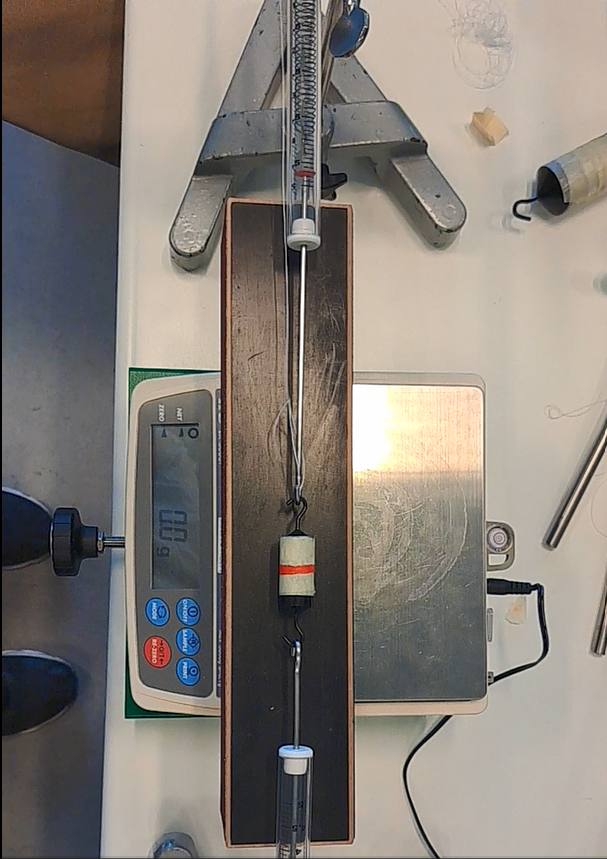
\includegraphics[width=0.7\linewidth, origin=c]{figures/video_eksempel.png}
    \caption{Snapshot fra en optagelse}
    \label{fig:optagelse}
\end{wrapfigure}
Vi udførte 2 forsøg med 3 gentagelser af hver. Det første var at vi optrækkede loddet til dens fuldt udspændte position og så slap den. 
Her varierede vi normalkraften hvormed underlaget trykkede på loddet. Vi gjorde det af 4 omgange. Først med en normalkraft på 0, altså intet underlag, så med en normalkraft under massen af loddet, en cirka ligmed massen af loddet, og en der var over.
Herefter gennemførte vi det samme forsøg, men ved cirka den halve startamplitude. Start amplituden var dog ikke så konsistent, som i det første, da det foregik ved øjemål, i modsætning til optrækningen i det første tilfælde, der stoppede når newtonmeteret ikke kunne strækkes mere ud.